% !TeX spellcheck = ru_RU
\chapter{Исследовательская часть}

%\section{Демонстрация работы программы}
% убрать секшн, мало обьема
	Демонстрация работы программы приведена на рисунке \ref{img:primer}.
\begin{figure}[h]
	\begin{center}
		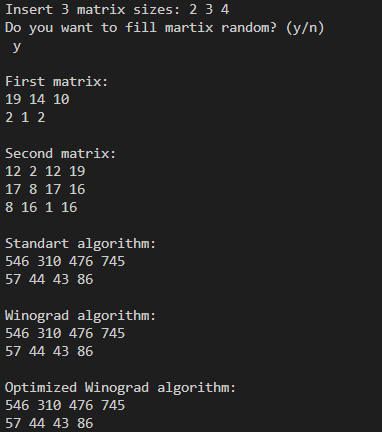
\includegraphics[scale=1]{example.png}
		\caption{Работа алгоритмов нахождения расстояний Левенштейна и Дамерау-Левенштейна.}
		\centering
		\label{img:primer}
	\end{center}
\end{figure}

\section{Технические характеристики}

Ниже приведены технические характеристики устройства, на котором было проведено измерение времени работы ПО:

\begin{itemize}
	\item операционная система Windows 10 Домашняя Версия 21H1 \cite{windows} x86\_64;
	\item оперативная память 8 Гб 2133 МГц;
	\item процессор Intel Core i5-8300H с тактовой частотой 2.30 ГГц \cite{intel}.
\end{itemize}

\section{Время выполнения реализаций алгоритмов}

Для замеров времени используется функция замера процессорного времени process\_time из библиотеки time на Python. Функция возвращает процессорное время типа float \cite{time}.

Функция используется дважды --- в начале и в конце замера времени, затем значения начальное значение вычитается из конечного.

Замеры проводились для слов длины от 0 до 9 раз на строках равной длины по 1000 раз. 

В таблице \ref{tbl:times} представлены замеры времени работы для каждого из алгоритмов.


\begin{table}[h]
	\captionsetup{justification=raggedright,singlelinecheck=off}
	\caption{Результаты замеров времени (в мс)}
	\label{tbl:times}
	\begin{tabular}{|c|c|c|c|c|}\hline%
		Длина & Лев.(матр.) & Д.-Л.(матр.)& Д.-Л.(рек.) & Д.-Л.(рек. с кэшем)
		\csvreader[head to column names]{csv/res.csv}{}%
		{\\ \hline\len & \lev & \dam & \damr & \damc}%
		\\ \hline
	\end{tabular}
\end{table}

На рисунках \ref{img:graph_levenshtein}, \ref{img:graph_damer}, \ref{img:graph_damer2} приведены графические результаты замеров.

% нету длины строки 2.5
\begin{figure}[h]
	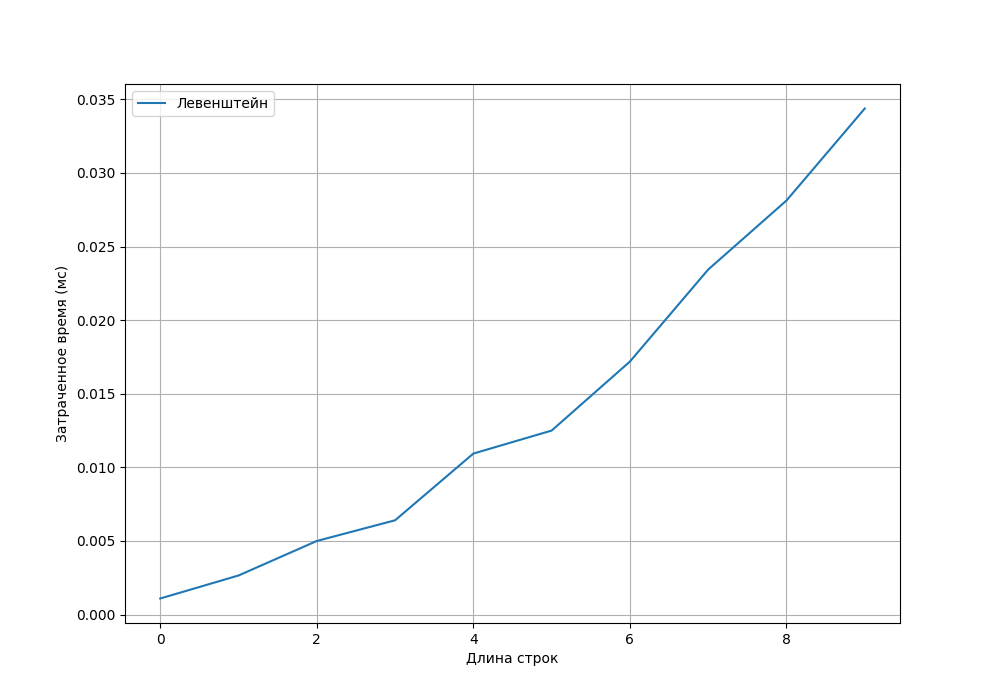
\includegraphics[scale = 0.55]{graph_levenshtein}
	\caption{Результаты работы алгоритма поиска расстояния Левенштейна для строк длины от 0 до 9}
	\centering
	\label{img:graph_levenshtein}
\end{figure}

% не закрыл скобку на картинке + лишнее заскриншотил
\begin{figure}[h]
	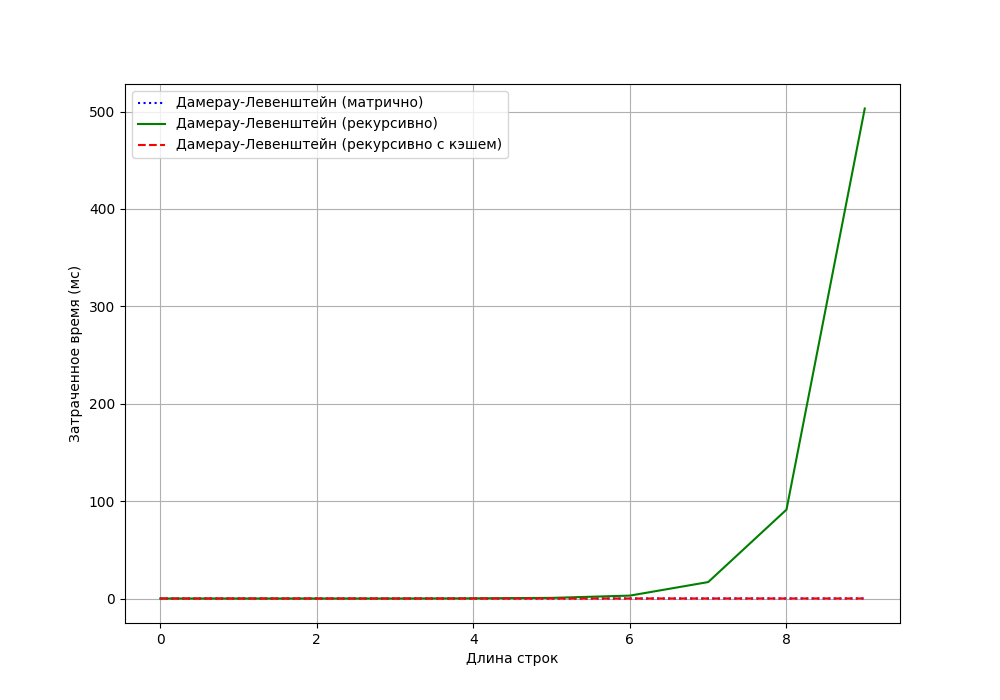
\includegraphics[scale = 0.65]{graph_damer}
	\caption{Сравнение результатов работы реализаций алгоритмов поиска расстояния Дамерау-Левенштейна для строк длины от 0 до 9}
	\centering
	\label{img:graph_damer}
\end{figure}

\begin{figure}[h]
	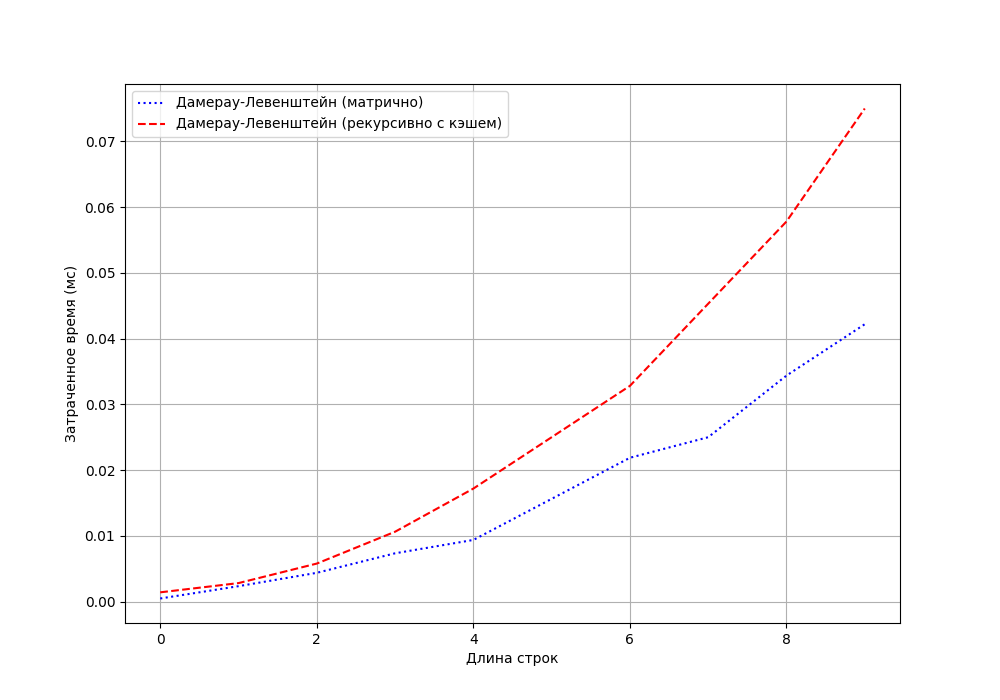
\includegraphics[scale = 0.65]{graph_damer2}
	\caption{Результаты работы реализаций алгоритмов поиска расстояния Левенштейна для строк длины от 0 до 9}
	\centering
	\label{img:graph_damer2}
\end{figure}
\clearpage

% рисунок ничего не показывает. Писать алгоритм имеет сложность... \ref{рисунок}
Из полученных результатов можно сделать вывод, что алгоритм поиска расстояния Левенштейна в общем случае имеет сложность $O(N^2)$ (рис. \ref{img:graph_levenshtein}).

Рекурсивная реализация поиска расстояния Дамерау-Левенштейна сильно уступает по временным характеристикам матричной реализации и реализации с кэшем (рис. \ref{img:graph_damer}).

\section{Использование памяти}

Алгоритмы нахождения расстояния Левенштейна и Дамерау—Левенштейна не отличаются друг от друга с точки зрения использования памяти.

\begin{itemize}
%зибавитсья от булетов
\item Для матричного алгоритма нахождения расстояния Левенштейна(Дамерау-Левенштейна) расходы памяти составляют:
% умножение вместо плюса в формуле памяти на матрицу
\begin{itemize}
	\item $sizeof(char)\cdot(n + m)$ --- для двух строк длин n и m
	\item $sizeof(int)\cdot((n + 1) \cdot (m + 1))$ --- для  матрицы промежуточных значений
	\item $sizeof(int)\cdot2$ --- для n и m
	\item $sizeof(int)\cdot2$ --- вспомогательные локальные переменные
	\item адрес возврата
\end{itemize}

\item Единоразовые расходы памяти для рекурсивной реализации:
\begin{itemize}
	\item $sizeof(char)\cdot(n + m)$ --- для двух строк длин n и m
\end{itemize}
Расходы памяти для каждого вызова функции рекурсивной реализации (максимум n + m вызовов): 

\begin{itemize}
	\item $sizeof(int)\cdot2$ --- для n и m
	\item $sizeof(int)\cdot1$ --- вспомогательная локальная переменная
	\item адрес возврата
\end{itemize}


Максимальные затраты памяти рекурсивного алгоритма достигаются при максимальной глубине рекурсии, равной сумме длин строк(n + m). Таким образом, теоретические максимальные затраты памяти рекурсивной реализации составляют $(sizeof(char)\cdot(n + m) + sizeof(int)\cdot3)\cdot(n + m) $

\item Также для рекурсивного алгоритма с кэшем следует учитывать единичные (не для каждого шага рекурсии, а только единожды) затраты памяти на хранение матрицы-кэша $((n + 1)\cdot(m + 1))\cdot sizeof(int))$
\end{itemize}


\section*{Вывод}

В результате экспериментов было выявлено, что обычный матричный алгоритм поиска расстояния Дамерау-Левенштейна сравним по затратам ресурсов с рекурсивной реализацией с использованием кэша, однако следует учитывать дополнительные затраты времени и памяти на многочисленные рекурсивные вызовы, делающие матричный алгоритм более эффективным по ресурсам.

Обычная рекурсивная реализация (без кэша) выигрывает у матричного метода по затратам памяти, т. к. максимальные затраты памяти рекурсивного варианта растут как функция от $(n + m)$, а у матричного варианта --- $(n+1)\cdot(m+1)$. Однако время выполнения рекурсивного варианта быстро растет и начинает многократно превосходить время выполнения матричной реализации уже начиная с длины строк равной 5.




